% This is the Latex template for my future homework write-ups
% A basic form of Latex command: '/command name[argu, argu]{argu*}' as below:
\documentclass[12pt, letterpaper]{article} % use 'tab' to complete 
% which means this document is an article with 12pt (font size) and letterpaper (paper type)


% ======================================================
% This is the preamble section for loading packages, a basic form looks like: 
% /usepackage{filename} the package name is the .sty file.  Let's load some 
% packages (Latex will complain if the .sty file is not in PWD):
% ======================================================
\usepackage{indentfirst} % indent the 1st line of the 1st paragraph, using \noindent to cancel
\usepackage{amsmath} % basic mathematic 
\usepackage{graphicx} % for using graphics
\usepackage{array} % for using arrays
\usepackage{lineno}   % for adding line numbers
\usepackage[authoryear]{natbib}   % for citing, more options see 'natbib'
\usepackage{bm}  % Use the bold mode in math 
\usepackage{ulem} % added lines for our text, i.e., underline...
\usepackage{xcolor} % used for adding color to our text
\usepackage{listings} % used for displaying the highlight code


% ============================================================================
% These are basic settings for making title and content
% ============================================================================
% Now, we start the work by entering the document with:
\begin{document}  % always remember 'begin - end' pairs
% Basic settings for the title page
\title{\LaTeX: Phys 5391 Assignment 4} % title name
\author{Yu Hong\\Space Physics Group} % double-slash for new line
\date{October 27, 2020}  % or the \today command to insert today's date.
% Now setting the format of the article
\maketitle % make a title based on  the info above


% ============================================================================
% This Section is used for "Program Description"
% ============================================================================
\section{Program Description} % Start a new section for figure

There are two python codes inside the Github folder for homework-4. The code named \textbf{weasel\_pro.py} is 
the function for calculating the generations required for reaching the target under the input offspring numbers and 
mutation rate; The code named \textbf{weasel\_script.py} is a script for testing the result, also, input the offspring 
numbers and mutation rate through command line.

 \textbf{weasel\_pro.py}  
 
this function named \textit{\textbf{offspring\_select}} is defined with inputs: target string, number of offspring along with mutation
rate and output: the generations required for reaching the target. Inside the function, firstly, we imported the modules used in this 
code: random and string; next, we defined the variables and parameters, such as the gene library, the new weasel child and parents;
then we created the first parents randomly. we started the main program with the whole loop: creating new generations. the termination 
signal is when the offspring reached the target. For the main program part, we separated into three sections: in the first section, we 
created mutated offspring, when the randomly outputted mutation rate is less than the given mutation rate, the child's gene will be 
replaced by a new 'letter' from the gene library; in the second section, according to the idea of "monkey print Shakespeare", we 
compared the digits of the offspring with the corresponding digits in the target, the key point is, we keep the most similar (with the 
defined difference variable) offspring as the new parent for the next round of generation, this process is the so-called “Natural Selection”; 
In the last section, we quantified the fitness of the most similar offspring in each generation with the target, and printed the offspring 
strings with and fitness, different digits with the target. In the output strings, we kept the correct digits as the corresponding genes in
the target and replaced the wrong digits with \* signs.
 
 \textbf{weasel\_script.py} 
 
 Inside this script, we first imported the function defined in the above python module, then we use "input" function to notice the 
 user to give inputs of offspring numbers and mutation rate; finally, we calculated the required generations and printed it on the screen.

% Package 'graphicx' is needed: already loaded
\graphicspath{ {./images/} } % Added the Figure path, or you can put it directly the same path with this code
This figure \textit{\textbf{Weasel Program}} is the running results from number of offspring of 5000 and mutation rate of 0.09,
the required generations is 17.

\begin{figure}[!t] % !b for bottom, t for top; ! for good position
\begin{center} % put the figure in the center 
  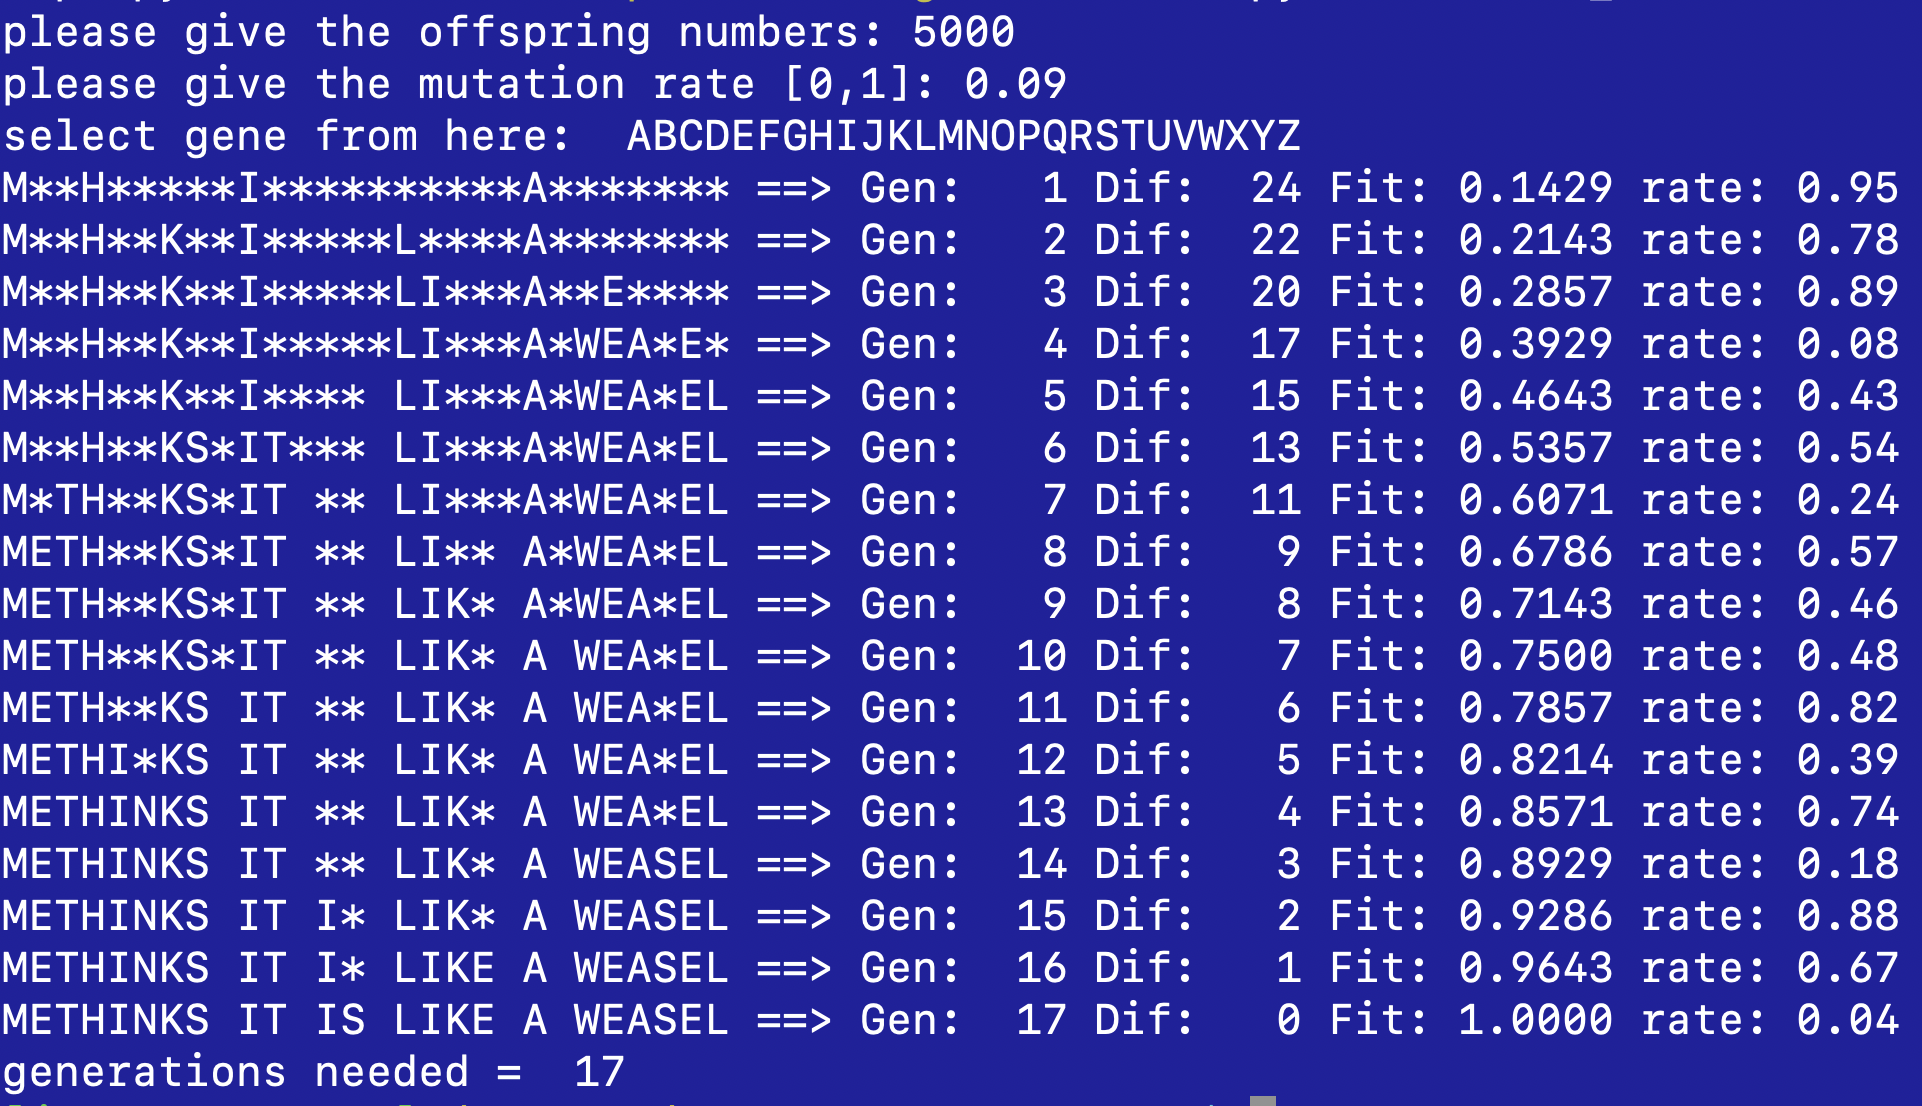
\includegraphics[width=12cm,height=6cm]{running_result.png} % changing figure size and rotate: scale=1.2, angle=45
  \caption{Weasel Program} % This figure is in the same path as the code
  \label{png:running_result} % label the figure with the unique name "rick"
\end{center} % end the environment {center}
\end{figure} % end the environment {figure}

% ============================================================================
% This Section is used for "Explore the Result"
% ============================================================================
\section{Explore the Result} % Start a new section for figure

Based on the program results, the generation size increases with decreasing offspring numbers and increasing mutation rate; 
while decreases with increasing offspring numbers and decreasing mutation rate. For example:

For 5000 offspring numbers and 0.01 mutation rate, the generation required is: ~30;

For 5000 offspring numbers and 0.09 mutation rate, the generation required is: ~70;

For 50 offspring numbers and 0.09 mutation rate, the generation required is: ~150;

The program is not always converged, when the offspring number is too small, e.g., 1 or the mutation rate is too big, e.g., 0.9,
the program will be killed.


% ============================================================================
% This Section is used for demonstrating some basic command of controlling Figures
% ============================================================================
\section{Imagination and Strategy} % Start a new section for figure

According to the basic information of "Weasel\_Program" and the python code:

1. A essential condition to ensure the target can be reached in most cases (properly offspring numbers and mutation rate) is
that the number of genes in the offspring should be the same as the target, that is, the gene at any position or digit can be 
changed in the reproduction process, but the number of genes cannot disappear or increase;

2. If we want to shorten the generation of reaching the target, we can add new limitation that when the most similarly offspring 
is used for the next generation, the correct gene digits will not change anymore; 

3. In selecting the most similar individual among the offspring in each generation and making it as the parent for the next 
generation, this follows the natural selection rule. It should be pointed out that, we assume that the most similarly individual
is directly used for reproducing the next generation (not hermaphrodite);

4. I got some idea from the "monkey print Shakespeare", since they both use comparison between the current result and the target 
result. But they are different: the monkey print can start from the first digit of the gene and compare and match the digits one by 
one; while for this program, the offspring should get the same gene digits at one time;

5. One important thing is that there should have a clear termination signal in the large whole loop of the program, that is, it stops when
the offspring reached the target;



\subsection{Links to my Github} % start a new subsection

\begin{quote} 
% The environment verbatim is used to print exactly what you type in
\begin{verbatim}
https://github.com/Yukiooooo/PHYS-5391/tree/master/assignment-4
\end{verbatim} % end the environment {verbatim}
\end{quote} % end the environment {quote}

All the introductions are in the README.md file. 


% End the document environment.  This is the last line for coding
\end{document}










